\documentclass{ximera}
\graphicspath{  %% When looking for images,
{./}            %% look here first,
{./pictures/}   %% then look for a pictures folder,
{../pictures/}  %% which may be a directory up.
{../../pictures/}  %% which may be a directory up.
{../../../pictures/}  %% which may be a directory up.
{../../../../pictures/}  %% which may be a directory up.
}

\usepackage{listings}
%\usepackage{circuitikz}
\usepackage{xcolor}
\usepackage{amsmath,amsthm}
\usepackage{subcaption}
\usepackage{graphicx}
\usepackage{tikz}
%\usepackage{tikz-3dplot}
\usepackage{amsfonts}
%\usepackage{mdframed} % For framing content
%\usepackage{tikz-cd}

  \renewcommand{\vector}[1]{\left\langle #1\right\rangle}
  \newcommand{\arrowvec}[1]{{\overset{\rightharpoonup}{#1}}}
  \newcommand{\ro}{\texttt{R}}%% row operation
  \newcommand{\dotp}{\bullet}%% dot product
  \renewcommand{\l}{\ell}
  \let\defaultAnswerFormat\answerFormatBoxed
  \usetikzlibrary{calc,bending}
  \tikzset{>=stealth}
  




%make a maroon color
\definecolor{maroon}{RGB}{128,0,0}
%make a dark blue color
\definecolor{darkblue}{RGB}{0,0,139}
%define the color fourier0 to be the maroon color
\definecolor{fourier0}{RGB}{128,0,0}
%define the color fourier1 to be the dark blue color
\definecolor{fourier1}{RGB}{0,0,139}
%define the color fourier 1t to be the light blue color
\definecolor{fourier1t}{RGB}{173,216,230}
%define the color fourier2 to be the dark green color
\definecolor{fourier2}{RGB}{0,100,0}
%define teh color fourier2t to be the light green color
\definecolor{fourier2t}{RGB}{144,238,144}
%define the color fourier3 to be the dark purple color
\definecolor{fourier3}{RGB}{128,0,128}
%define the color fourier3t to be the light purple color
\definecolor{fourier3t}{RGB}{221,160,221}
%define the color fourier0t to be the red color
\definecolor{fourier0t}{RGB}{255,0,0}
%define the color fourier4 to be the orange color
\definecolor{fourier4}{RGB}{255,165,0}
%define the color fourier4t to be the darker orange color
\definecolor{fourier4t}{RGB}{255,215,0}
%define the color fourier5 to be the yellow color
\definecolor{fourier5}{RGB}{255,255,0}
%define the color fourier5t to be the darker yellow color
\definecolor{fourier5t}{RGB}{255,255,100}
%define the color fourier6 to be the green color
\definecolor{fourier6}{RGB}{0,128,0}
%define the color fourier6t to be the darker green color
\definecolor{fourier6t}{RGB}{0,255,0}

%New commands for this doc for errors in copying
\newcommand{\eigenvar}{\lambda}
%\newcommand{\vect}[1]{\mathbf{#1}}
\renewcommand{\th}{^{\text{th}}}
\newcommand{\st}{^{\text{st}}}
\newcommand{\nd}{^{\text{nd}}}
\newcommand{\rd}{^{\text{rd}}}
\newcommand{\paren}[1]{\left(#1\right)}
\newcommand{\abs}[1]{\left|#1\right|}
\newcommand{\R}{\mathbb{R}}
\newcommand{\C}{\mathbb{C}}
\newcommand{\Hilb}{\mathbb{H}}
\newcommand{\qq}[1]{\text{#1}}
\newcommand{\Z}{\mathbb{Z}}
\newcommand{\N}{\mathbb{N}}
\newcommand{\q}[1]{\text{``#1''}}
%\newcommand{\mat}[1]{\begin{bmatrix}#1\end{bmatrix}}
\newcommand{\rref}{\text{reduced row echelon form}}
\newcommand{\ef}{\text{echelon form}}
\newcommand{\ohm}{\Omega}
\newcommand{\volt}{\text{V}}
\newcommand{\amp}{\text{A}}
\newcommand{\Seq}{\textbf{Seq}}
\newcommand{\Poly}{\textbf{P}}
\renewcommand{\quad}{\text{    }}
\newcommand{\roweq}{\simeq}
\newcommand{\rowop}{\simeq}
\newcommand{\rowswap}{\leftrightarrow}
\newcommand{\Mat}{\textbf{M}}
\newcommand{\Func}{\textbf{Func}}
\newcommand{\Hw}{\textbf{Hamming weight}}
\newcommand{\Hd}{\textbf{Hamming distance}}
\newcommand{\rank}{\text{rank}}
\newcommand{\longvect}[1]{\overrightarrow{#1}}
% Define the circled command
\newcommand{\circled}[1]{%
  \tikz[baseline=(char.base)]{
    \node[shape=circle,draw,inner sep=2pt,red,fill=red!20,text=black] (char) {#1};}%
}

% Define custom command \strikeh that just puts red text on the 2nd argument
\newcommand{\strikeh}[2]{\textcolor{red}{#2}}

% Define custom command \strikev that just puts red text on the 2nd argument
\newcommand{\strikev}[2]{\textcolor{red}{#2}}

%more new commands for this doc for errors in copying
\newcommand{\SI}{\text{SI}}
\newcommand{\kg}{\text{kg}}
\newcommand{\m}{\text{m}}
\newcommand{\s}{\text{s}}
\newcommand{\norm}[1]{\left\|#1\right\|}
\newcommand{\col}{\text{col}}
\newcommand{\sspan}{\text{span}}
\newcommand{\proj}{\text{proj}}
\newcommand{\set}[1]{\left\{#1\right\}}
\newcommand{\degC}{^\circ\text{C}}
\newcommand{\centroid}[1]{\overline{#1}}
\newcommand{\dotprod}{\boldsymbol{\cdot}}
%\newcommand{\coord}[1]{\begin{bmatrix}#1\end{bmatrix}}
\newcommand{\iprod}[1]{\langle #1 \rangle}
\newcommand{\adjoint}{^{*}}
\newcommand{\conjugate}[1]{\overline{#1}}
\newcommand{\eigenvarA}{\lambda}
\newcommand{\eigenvarB}{\mu}
\newcommand{\orth}{\perp}
\newcommand{\bigbracket}[1]{\left[#1\right]}
\newcommand{\textiff}{\text{ if and only if }}
\newcommand{\adj}{\text{adj}}
\newcommand{\ijth}{\emph{ij}^\text{th}}
\newcommand{\minor}[2]{M_{#2}}
\newcommand{\cofactor}{\text{C}}
\newcommand{\shift}{\textbf{shift}}
\newcommand{\startmat}[1]{
  \left[\begin{array}{#1}
}
\newcommand{\stopmat}{\end{array}\right]}
%a command to give a name to explorations and hints and theorems
\newcommand{\name}[1]{\begin{centering}\textbf{#1}\end{centering}}
\newcommand{\vect}[1]{\vec{#1}}
\newcommand{\dfn}[1]{\textbf{#1}}
\newcommand{\transpose}{\mathsf{T}}
\newcommand{\mtlb}[2][black]{\texttt{\textcolor{#1}{#2}}}
\newcommand{\RR}{\mathbb{R}} % Real numbers
\newcommand{\id}{\text{id}}
\newcommand{\coord}[1]{\langle#1\rangle}
\newcommand{\RREF}{\text{RREF}}
\newcommand{\Null}{\text{Null}}
\newcommand{\Nullity}{\text{Nullity}}
\newcommand{\Rank}{\text{Rank}}
\newcommand{\Col}{\text{Col}}
\newcommand{\Ef}{\text{EF}}
\newcommand{\boxprod}[3]{\abs{(#1\times#2)\cdot#3}}


\author{Zack Reed}
%borrowed from Dirk Colbry's msu python stuff
\title{Rank and Nullity}
\begin{document}
\begin{abstract}

In this activity, we will explore the rank and nullity of a matrix.

\end{abstract}
\maketitle

\section*{Null Spaces: Mapping to $\vec{0}$}

\begin{exploration}

    Let's start with a little warm up exploration! We'll think in $\mathbb{R}^2$ for now.
    
    Remember that linear transformations are completely determined by where they send the standard basis vectors ($\vec{i}$ and $\vec{j}$ for $\mathbb{R}^2$), and that it's possible to determine $\vec{i}$ and $\vec{j}$ such that you can't span all of $\mathbb{R}^2$ from result of the transformation.

    Go back to the 2D linear transformation GeoGebra applet from before and set $S(\vec{i})$ and $S(\vec{j})$ such that the transformation $S$ only gives you a 1-dimensional subspace of $\mathbb{R}^2$ (i.e. a line).
    
    \geogebra{uaua5mpa}{1156}{636}

    Now, we're going to try to answer a very specific question in this section: What vectors get mapped to $\vec{0}$ by a matrix $A$? Remember that all linear transformations are matrices, so we can reprsent this in the applet by finding vectors $\vec{v}$ such that $S(\vec{v})=\vec{0}$.

    This should be simple enough in the applet, if you set up $S(\vec{i})$ and $S(\vec{j})$ correctly you should be able to hone in on such vectors by rotating $\vec{v}$ around the origin.

    Once you pick up on a few vectors such that $S(\vec{v})=\vec{0}$, try to describe the set of all such vectors. What do you notice about them? Is the set of all such vectors an eclectic collection, or is there a pattern?

    \begin{solution}

        One example is to set $S(\vec{i})=\begin{bmatrix} 1 \\ -1 \end{bmatrix}$ and $S(\vec{j})=\begin{bmatrix} -1 \\ 1 \end{bmatrix}$. The $S$ maps $\RR^2$ to the line $y=-x$. Vectors $\vec{v}$ whose coordinates are the same, such as $\begin{bmatrix} .38 \\ .38 \end{bmatrix}$ in the figure below, get mapped to $\vec{0}$. Otherwise, vectors get mapped to points on the line $y=-x$. 

        %insert figure
        \begin{center}
            \includegraphics[scale=.25]{null_space_1.png}
        \end{center}
    
        In fact, all vectors whose coordinates agree lie along the line $y=x$, so we've found that only vectors within the 1-dimensional subspace spanned by $\begin{bmatrix} 1 \\ 1 \end{bmatrix}$ get mapped to $\vec{0}$. This is an example of what's called a \emph{null space} of a matrix, which we'll explore more in the next few problems.

    \end{solution}

\end{exploration}

Let's start to more systematically explore the idea of a null space in $\mathbb{R}^3$.

Consider the following matrix $A$. 

$$ 
\left[
\begin{matrix}
    1 & 0 & 3  \\
    0 & 1 & 5  \\
    1 & 1 & 8 
\end{matrix}
\right] 
$$

\begin{remark}

    Notice that the third column of $A$ is a linear combination of the first two columns!

    While we can determine this by 
    
    \[3\begin{bmatrix}1\\0\\1\end{bmatrix}+5\begin{bmatrix}0\\1\\1\end{bmatrix}=\begin{bmatrix}3\\5\\8\end{bmatrix},\]

    let's also practice our echelon form skills. 

    In MATLAB, if we take the \rref of $A$ by:

    \begin{verbatim}
        A=[1, 0, 3;
            0, 1, 5;
            1, 1, 8]
        A=sym(A)

        rref(A)
    \end{verbatim}

    We get $\text{rref}(A)=\begin{bmatrix}1&0&3\\0&1&5\\0&0&0\end{bmatrix}$

    This gives us the exact same information! In fact, in cases like this, the \rref will tell us what linear combinations of the first two columns equals the third!
    
    In other words, $A\vec{k}$ is in the span of $A\vec{i}$ and $A\vec{j}$. This is a hint that $A$ doesn't give you all of $\mathbb{R}^3$. 

    Let's view this in our handy GeoGebra applet to confirm where $A$ sends 3D vectors.

    \begin{center}
    
        \geogebra{gseknqrg}{954}{599}

    \end{center}

    In fact, after setting up the matrix, it's clear that the vector $A\vec{v}$ always stays on the plane spanned by $\begin{bmatrix}1\\0\\1\end{bmatrix}$ and $\begin{bmatrix}0\\1\\1\end{bmatrix}$. No matter where you place $\vec{v}$, $A\vec{v}$ always stays on the plane. 

\end{remark}


%\begin{problem}{{\bf Warm Up:}}
%    What is the reduced row echelon form of $A^T$? This will tell you which %vectors span the $Im(A)$ (i.e. ``the image of $A$").
%    \begin{solution}
%        Since reduced row echelon usually operates with rows, we take the %transpose of $A$ to instead talk about its columns, which we've come to %primarily associate with the $Im(A)$.
%        \[
%            A^T = 
%            \begin{bmatrix}
%            1 & 0 & 1 \\
%            0 & 1 & 1 \\
%            3 & 5 & 8
%            \end{bmatrix}
%            \]
%
%        As we said, we can combine the first two rows to generate the third row, %so the reduced row echelon form of $A^T$ is%
%
%        \[
%            \begin{bmatrix}
%            1 & 0 & 1 \\
%            0 & 1 & 1 \\
%            0 & 0 & 0
%            \end{bmatrix}
%        \]

%        This confirms that $Im(A)$ is spanned by $\begin{bmatrix} 1 \\ 0 \\ 1 %\end{bmatrix}$ and $\begin{bmatrix} 0 \\ 1 \\ 1 \end{bmatrix}$.
%
%        In the next few examples, we'll provide some commands to help you find %the reduced row echelon form of more complicated matrices.
%    \end{solution}

%\end{problem}

\subsection*{The Image of a Linear Transformation}

\begin{remark}{Issues with Learning Math: Ambiguity, Many Names for the Same Thing, Many Meanings for the Same Word}

  One of the things that you have to get used to in math is the hyper-contextual meanings of words. 

  Often in math, depending on the context, many terms are used for what is more or less the same thing. This is exacerbated when you add in domains like physics, chemistry, and data science. 

  Other times, very much depending on the context, the same word is used to mean many different things, sometimes within the same problem. ``Normal'' is the most eggregious offender of this. Off the top of my head I can think of at least four different meanings for ``normal'', depending on the context.

  Such is the case when it comes to linear transformations and matrices. Expect to run into the ``many names for the same thing'' phenomenon here. 

\end{remark}

Remembering that any time we talk about \emph{linear transformations} in this class, we're also talking about \emph{matrices} that send vectors from one vector space $V$ to another vector space $W$, let's dig into the weeds of some terminology.

It's becoming cumbersome to always say ``A maps vectors $\vec{v}$ to a line'', or ``the vector $\vec{v}$ gets mapped to the vector $A\vec{v}$'', so we come up with succinct terminology to describe mapping and being mapped. 

\begin{definition}\label{def:imageofT}
Let $V$ and $W$ be vector spaces, and let $T:V\rightarrow W$ be a linear transformation.  The \dfn{image} of $T$, denoted by $\mbox{im}(T)$, is the set
$$\mbox{im}(T)=\{T(\vec{v}):\vec{v}\in V\}$$
In other words, the image of $T$ consists of individual vectors $T(\vec{v})$ mapped to in $W$.
\end{definition}
 
\begin{example}\label{ex:image1}
Consider the matrix
$$A=\begin{bmatrix}1&2&3\\2&4&6\end{bmatrix}.$$

$A$ defines a linear transformation $T$, let's find and illustrate $\mbox(im)(T)$.
 

First, let's see what $A$ does to an arbitrary vector $\vec{v}=\begin{bmatrix}a\\b\\c\end{bmatrix}$.
 
$$A\vec{v}=\begin{bmatrix}1&2&3\\2&4&6\end{bmatrix}\begin{bmatrix}a\\b\\c\end{bmatrix}=a\begin{bmatrix}1\\2\end{bmatrix}+b\begin{bmatrix}2\\4\end{bmatrix}+c\begin{bmatrix}3\\6\end{bmatrix}$$
 
So far, we've re-stated little more than the definition of matrix-vector multiplication, but it's good to remember that matrix-vector multiplication gives us linear combinations of the column vectors of $A$. And now, in our new language, we state that $\mbox(im)(T)$ for any matrix $A$ is always a linear combination of the column vectors!

Let's dig further to better describe this particular image. 

If we take \texttt{rref(A)}, we get

$$\text{rref}(A)=\begin{bmatrix}1&2&3\\0&0&0\end{bmatrix}.$$

Like we just discussed, this means that the second two column vectors are actually linear combiantions of the first column vector!

So really the entire image of $T$ is just linear combinations of the vector $\begin{bmatrix}1\\2\end{bmatrix}$, which we know as a line, depicted below.
 
\begin{center}
    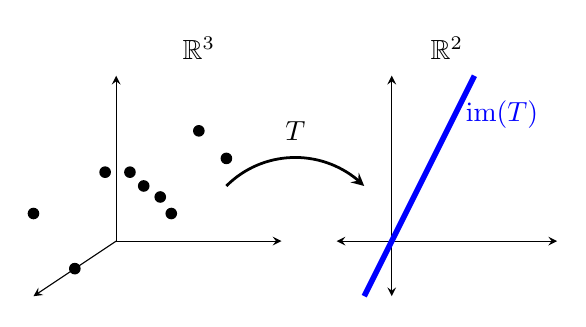
\begin{tikzpicture}[scale=.7]
     
      % Left image
      \node at (1.5, 3.5) {$\mathbb{R}^3$}; % Title for the left image
      \draw[->] (0,0)--(3,0); % x-axis
      \draw[->] (0,0)--(0,3); % y-axis
      \draw[->] (0,0)--(-1.5,-1); % diagonal axis
    
      % Random multicolored points in the left image
      \foreach \x/\y/\color in {0.5/1/red, 1/0.5/green, 1.5/2/blue, 2/1.5/orange, 0.8/0.8/purple, -1.5/.5/red, -.75/-.5/blue, -.2/1.25/red, .25/1.25/orange} {
        \fill[\color] (\x, \y) circle (3pt);
      }
      
      % Right image
      \node at (6, 3.5) {$\mathbb{R}^2$}; % Title for the right image
      \draw[<->] (4,0)--(8,0); % x-axis
      \draw[<->] (5,-1)--(5,3); % y-axis
      \draw[line width=2pt,blue] (4.5,-1)--(6.5,3); % diagonal line
    
      % Labels
      \node[] at (3.25, 2) (b) {$T$};
      \draw [->,line width=1pt,-stealth] (2,1) to[out=45] (4.5, 1);
      \node[blue] at (7, 2.3) (b) {$\mbox{im}(T)$};
     
    \end{tikzpicture}
\end{center}

As we suspected, the matrix sends $3-$dimensional vectors to $2-$dimensional vectors, which happen to all live on the same line.

\end{example}

\begin{remark}{Images and Pre-Images}
Up to this point we've been focusing mainly on the image of matrices and their properties, but we can actually say much about a matrix in terms of the \emph{pre-image} space. The pre-image space is the set of all vectors $\vec{v}$ that get mapped by $A$ into the image $A\vec{v}$. 

\begin{definition}
    The \emph{pre-image} of a function or transformation is the set of all vectors $\vec{v}$ such that $T(\vec{v})$ is defined.
\end{definition}

\begin{example}

    The matrix 
    
    $$M=\begin{bmatrix}1,1,0\\0,1,1\\-1,1,1\end{bmatrix}$$
    
    is a $3\times 3$ matrix. So any $3-$dimensional vector $\vec{v}$ is in the pre-image of $M$, since $M\vec{v}$ is defined, however $2-$ or $4-$dimensional vectors $\vec{u}$ and $\vec{w}$ are not in the pre-image of $M$, since $A\vec{u}$ and $A\vec{w}$ would not be defined.

\end{example}

One way to describe why the $Im(A)$ is just a plane is to note that some pre-image vectors get mapped to $\vec{0}$. As it turns out, the set of all vectors that get mapped to $\vec{0}$ is a subspace of $\mathbb{R}^3$. We call it the \emph{null space} of $A$.

\end{remark}

Let's go back to our simple diagram that conveys the basic concept of mapping vectors.

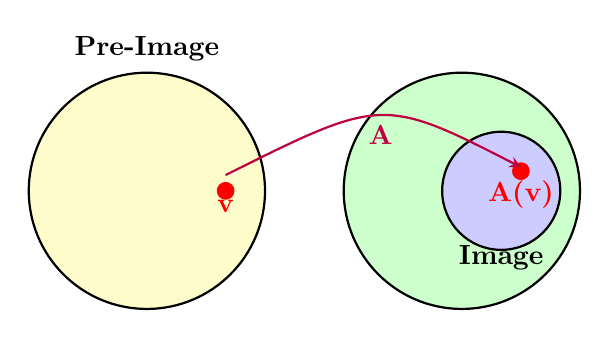
\begin{tikzpicture}

    % Draw sets A, B, C
    \draw[fill=yellow!20!white, draw=black, thick] (-4,0) ellipse (1.5cm);
    \draw[fill=green!20!white, draw=black, thick] (0,0) ellipse (1.5cm);
    \draw[fill=blue!20!white, draw=black, thick] (.5,0) ellipse (.75cm);
    
    % Labels for sets A, B, C
    \node at (-4,1.8) {\textbf{Pre-Image}};
    \node at (.5,-.85) {\textbf{Image}};
    %\node at (4,1.8) {\textbf{X''}};
    
    % Elements inside sets
    \filldraw[red] (-3,0) circle (3pt) node[below] {\textbf{v}};
    \filldraw[red] (.75,.25) circle (3pt) node[below] {\textbf{A(v)}};
    %\filldraw[red] (3.5,-.5) circle (3pt) node[below] {\textbf{R(S(v))}};
    
    % Arrows for functions f, g, gof
    \draw[->, thick, purple] (-3,0.2) .. controls (-1,1.2) .. (.75,.3) node[midway, below] {\textbf{A}};
    %\draw[->, thick, purple] (1,.7) .. controls (2,1.5) .. (3.5,-.3) node[midway, above] {\textbf{R}};
    %\draw[->, thick, purple] (-4,-1.7) .. controls (0,-2.5) .. (4,-1.7) node[midway, below] {\textbf{RoS}};
    
\end{tikzpicture}

Now let's more formally define the \emph{null space} of $A$.

\begin{definition}

    The {\bf null space} of a matrix $A$ is the set of all vectors $\vec{v}$ such that $A\vec{v} = \vec{0}$. In more compact notation, we write this as 
    $$\text{Null}(A) = \{ \vec{v} \in \mathbb{R}^3 : A\vec{v} = \vec{0} \}.$$

    \begin{hint}

        Remember that in compact math notation, $\in$ reads "in" and $:$ reads |such that". So in words, $$\text{Null}(A) = \{ \vec{v} \text{ in } \mathbb{R}^3 \text{ such that } A\vec{v} = \vec{0} \}.$$

        Remember that $A\vec{v}$ gives you a vector, because the matrix $A$ is a linear transformation that sends vectors to vectors.

    \end{hint}

\end{definition}

\begin{remark}{Terminology Alert!}

    When we use the language of transformations $T$ instead of matrices $A$, we use the word \emph{kernel} instead of \emph{null space}.

    So the \emph{kernel} of the linear transformation $T$ is the \emph{null space} of its associated matrix, $A$.

    We also talk about the \emph{domain} as the space being mapped from (aka the pre-image) and then the \emph{co-domain} as the space being mapped \emph{to}. The co-domain and image distinction is more important, since the image is {\bf only} where the matrix sends vectors, whereas the co-domain is the ambient space in which the mapped vectors live. 

    In our example of $A=\begin{bmatrix}1&2&3\\2&4&6\end{bmatrix}$, the $\mbox{im}(A)$ was the line $\text{span}\left(\begin{bmatrix}1\\2\end{bmatrix}\right)$, whereas the co-domain was just $\RR^2$ since we were looking at $2-$dimensional vectors. 

    In this next image, $V$ is the domain (or pre-image), $W$ is the co-domain, and the smaller ellipse within $W$ labeled $\mbox{im}(T)$ is the image. Then, note, a blue subset of $V$ gets all mapped to $\vec{0}$. This would be the kernel of $T$, which is the same as the \emph{null space} of $A$.

    \begin{center}
        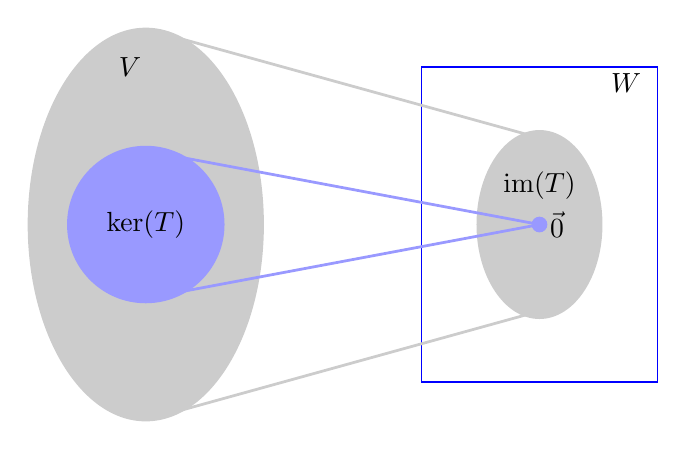
\begin{tikzpicture}
        \fill[gray!40] (0,0) ellipse (1.5cm and 2.5cm);
        \fill[blue!40!white] (0,0) ellipse (1cm and 1cm)node[black]{$\mbox{ker}(T)$};
         
        \draw[blue] (3.5,2) rectangle (6.5,-2);
        \node[] at (6.1, 1.8)   (b) {$W$};
        \fill[gray!40] (5,0) ellipse (0.8cm and 1.2cm);
        \fill[blue!40!white] (5,0) circle (0.1cm);
         
        \draw[gray!40,line width=1pt](0.3,2.4)--(5,1.1);
        \node[] at (-0.2, 2)   (b) {$V$};
        \node[] at (5, 0.5)   (b) {$\mbox{im}(T)$};
        \draw[gray!40, line width=1pt](0.3,-2.4)--(5,-1.1);
         
        \draw[blue!40!white, line width=1pt](0.2,.9)--(5,0);
        \draw[blue!40!white, line width=1pt](0.2,-0.9)--(5,0)node[below, right][black]{$\vec{0}$};
         
        \end{tikzpicture}
    \end{center}

\end{remark}


We have the following similar definition for \emph{kernel}:

\begin{definition}
    Let $V$ and $W$ be vector spaces, and let $T:V\rightarrow W$ be a linear transformation.  The \dfn{kernel} of $T$, denoted by $\mbox{ker}(T)$, is the set
    $$\mbox{ker}(T)=\{\vec{v}:T(\vec{v})=\vec{0}\}$$
    In other words, the kernel of $T$ consists of all vectors of $V$ that map to $\vec{0}$ in $W$.
\end{definition}

We'll mostly use the terminology Null Space, instead of Kernel, but at times kernel may arise. 

Now, armed with new terminology, let's see more how to find the null spaces of matrices. 

\begin{exploration}{Finding the Null Space of $A$}

Let's think back to how $A$ maps vectors as a linear transformation, and rearrange some variables to figure out how we determine which vectors $\vec{v}$ get mapped to $\vec{0}$. 

With our sample matrix $A=\begin{bmatrix} 1 & 0 & 3 \\ 0 & 1 & 5 \\ 1 & 1 & 8 \end{bmatrix}$, we want to find all vectors $\vec{v} = \begin{bmatrix} v_1 \\ v_3 \\ v_3 \end{bmatrix}$ such that $A\vec{v} = \vec{0}$.

This gives the systme of equations

%write the system with v_1, v_2, v_3
\[
\begin{aligned}
    1v_1 + 0v_2 + 3v_3 &= 0 \\
    0v_1 + 1v_2 + 5v_3 &= 0 \\
    1v_1 + 1v_2 + 8v_3 &= 0
\end{aligned}
\]

and the augmented matrix

\[A_a=\left[\begin{array}{ccc|c}1&0&3&0\\
    0&1&5&0\\
    1&1&8&0
\end{array}\right]\]

Using MATLAB as above, we get

$$A=\begin{bmatrix} 1 & 0 & 3 \\ 0 & 1 & 5 \\ 1 & 1 & 8 \end{bmatrix}$$

$$\text{rref}(A)=\begin{bmatrix} 1 & 0 & 3 \\ 0 & 1 & 5 \\ 0 & 0 & 0 \end{bmatrix}$$

This tells us that $v_3$ is a free variable. When $v_3=1$, we get the system 

\[
\begin{aligned}
    v_1 + 3v_3 &= v_1+3&=0 \\
    v_2 + 5v_3 &= v_2+5&=0
\end{aligned}
\]

which is only solved when $v_1=-3$ and $v_2=-5$. Therefore, the vector $\begin{bmatrix} -3 \\ -5 \\ 1 \end{bmatrix}$ gets mapped to $\vec{0}$.

In fact, any scalar multiple of this vector gets mapped to $\vec{0}$ as well, so if we generally let $v_3=\tau$, then we've determined that any vector of the form $\tau \begin{bmatrix} -3 \\ -5 \\ 1 \end{bmatrix}$ gets mapped to $\vec{0}$. 

We've found the null space! $Null(A)$ is the set of all vectors of the form $\tau \begin{bmatrix} -3 \\ -5 \\ 1 \end{bmatrix}$.

\end{exploration}

\begin{remark}

    The collection of the form $\tau \begin{bmatrix} -3 \\ -5 \\ 1 \end{bmatrix}$ is exactly the span of the vector $\begin{bmatrix} -3 \\ -5 \\ 1 \end{bmatrix}$, so we haven't just found the null space of $A$, we've also explicitly described $Null(A)$ as the span of a single vector.

    So, more specifically, we can say that $Null(A)=\text{span}\left\{ \begin{bmatrix} -3 \\ -5 \\ 1 \end{bmatrix} \right\}$. In other words, $\begin{bmatrix} -3 \\ -5 \\ 1 \end{bmatrix}$ is the single basis vector for the null space of $A$, and so $Null(A)$ is a one-dimensional subspace of $\mathbb{R}^3$.

\end{remark}

\begin{problem}{Testing the Null Space}

Let's make sure we're not off base! Pick a few scalars, say $\tau=\pi$ and $\tau=e$, and calculate the product $A\left(\tau\begin{bmatrix} -3 \\ -5 \\ 1 \end{bmatrix}\right)$. What do you get?

\begin{solution}

    We can use MATLAB to calculate the product $A\left(\tau\begin{bmatrix} -3 \\ -5 \\ 1 \end{bmatrix}\right)$ for $\tau=\pi$ and $\tau=e$.

    \begin{hint}{MATLAB Code}
    %\revealbutton{Click to see MATLAB code}
        %Write A as a matrix in MATLAB in a verbatim environment
        \begin{verbatim}
            A = [1 0 3; 
                0 1 5; 
                1 1 8]
            v=[-3; -5; 1]
            tau = pi;
            A_pi_v=A*(tau*v)
            
            tau = exp(1);
            A_e_v=A*(tau*v)
        \end{verbatim}
    \end{hint}

    Doing so yields

    $$A\left(\pi\vec{v}\right)=\begin{bmatrix} 0 \\ 0 \\ 0 \end{bmatrix}$$

    $$A\left(e\vec{v}\right)=\begin{bmatrix} 0 \\ 0 \\ 0 \end{bmatrix}$$

    MATLAB can also handle general scalars, so with the code


    \begin{verbatim}
        syms tau
        A_tau_v=A*(tau*v)
    \end{verbatim}

    we get the output

    $$A\left(\tau\vec{v}\right)=\begin{bmatrix} 0 \\ 0 \\ 0 \end{bmatrix}$$
    

\end{solution}

\end{problem}

As it turns out, this process will let you exactly determine the null space for any given matrix, no matter how nice or complex. Let's try it out with a more complicated matrix, $B$, but we'll shortcut the interlude with systems of equations and instead only work with the reduced row echelon form and the known pivots.

\begin{problem}{Finding the Null Space of $B$}

    %write the matrix B
    Let's consider the matrix $B=\begin{bmatrix}
        1 & 3 & 2 & 0 & 0  \\
        0 & 1 & 5 & 2 & 1  \\
        3 & 5 & -14 & -8 &-4  \\
        0 & 0 & 0 & 1 & 1  \\
        \end{bmatrix}$.

    Find a basis for the null space of $B$.

    \begin{solution}

        Let's start with the reduced row echelon form of $B$, but we're going to get a new output from \texttt{rref(B)}, which will tell us which columns are the pivot columns.

        (REMEMBER: The pivot columns refer to Gaussian Elimination, where you have leading 1s)

       %Write B as a matrix in MATLAB in a verbatim environment
       \begin{verbatim}
        B = [1 3 2 0 0; 
            0 1 5 2 1; 
            3 5 -14 -8 -4; 
            0 0 0 1 1]
        [R_new, pivcol_new]=rref(B)
    \end{verbatim}

        This generates the output
        
        \[
            B=\begin{bmatrix}
                1 & 0 & -13 & 0 & 3 \\
                0 & 1 & 5 & 0 & -1 \\
                0 & 0 & 0 & 1 & 1 \\
                0 & 0 & 0 & 0 & 0 \\
            \end{bmatrix}
        \]


    $$\text{pivcol\_new}=\begin{bmatrix} 1 & 2 & 4 \end{bmatrix}$$

    Since the pivot columns determine the solution variables (in this case $v_1, v_2, v_4$), the free variables are $v_3$ and $v_5$. 

    Since $B$ is a $4\times 5$ matrix, it maps 5D vectors to 4D vectors. Hence, the input vectors $\vec{v}$ for any product $B\vec{v}$ must be 5D vectors.

    Since $v_3$ and $v_5$ are free variables, we find the null space spanning vectors by setting each to $1$, the other variable to $0$, and solving for any remaining variables, as we did before.

    For instance, if $v_3=1$ and $v_5=0$, we get the system

    \[
    \begin{aligned}
        v_1 - 13v_3 + 3v_5 &= v_1 - 13 + 0 &= 0 \\
        v_2 + 5v_3 - v_5 &= v_2 + 5 - 0 &= 0 \\
        v_4 + v_5 &= v_4 + 0 &= 0
    \end{aligned}
    \]

    So one basis vector for the nullspace is $\begin{bmatrix} 13 \\ -5 \\ 1 \\ 0 \\ 0 \end{bmatrix}$.

    If we set $v_3=0$ and $v_5=1$, we get the null space basis vector $\begin{bmatrix} -3 \\ 1 \\ 0 \\ -1 \\ 1 \end{bmatrix}$.

    So, $Null(B)=\text{span}\left\{ \begin{bmatrix} 13 \\ -5 \\ 1 \\ 0 \\ 0 \end{bmatrix}, \begin{bmatrix} -3 \\ 1 \\ 0 \\ -1 \\ 1 \end{bmatrix} \right\}$.

    \end{solution}

\end{problem}

\begin{problem}

    Let's again test that we've found the right spanning vectors for the $Null(B)$.

    Ideally, linear combinations of the two vectors $\vec{v}=\startmat{c}13\\-5\\1\\0\\0\stopmat$ and $\vec{u}=\startmat{c}-3\\1\\0\\-1\\1\stopmat$ would map to $\vec{0}$.

    We can set this up by defining the matrix $A$, the vectors $\vec{v}$ and $\vec{w}$, and then arbitrary scalars $\tau$ and $\sigma$.

    \begin{verbatim}
        B = [1 3 2 0 0; 
            0 1 5 2 1; 
            3 5 -14 -8 -4; 
            0 0 0 1 1]
        B=sym(B)

        v=[13;-5;1;0;0]
        w=[-3;1;0;-1;1]

        syms tau sigma
        B*(tau*v+sigma*w)
    \end{verbatim}

    In fact, this yields $\vec{0}$, and so do the individual products $B\left(\tau \vec{v}\right)$ and $B\left(\sigma\vec{w}\right)$. Indeed, we've found our null space. 

    Or have we? We'll later see conditions by which we can be sure we've exhaustively found our null space, so let's table our certainty and come back to that question. In math, you always want to make sure you've set up the problem so that you can be certain of the result!

\end{problem}

\begin{remark}

    You might notice that a quick way to find the null space basis vectors is to set each free variable to $1$ and to negate any other elements in the column. This is a quick way to play out the implications of setting each free variable to $1$ and the others to $0$, as we did in the last problem.

    For example, if the reduced row echelon form of $C=\begin{bmatrix} 1 & 2 & 3 & 5 \\ 2 & 1 & 4 &2 \\ 5 & 4 & 11 & 9 \end{bmatrix}$ is 

    $$\text{rref}(C)=\begin{bmatrix} 1 & 0 & 5/3 & -1/3 \\ 0 & 1 & 2/3 & 8/3 \\ 0 & 0 & 0 & 0 \end{bmatrix}$$

    then the null space basis vectors are $\begin{bmatrix} -5/3 \\ -2/3 \\ 1 \\ 0 \end{bmatrix}$ and $\begin{bmatrix} 1/3 \\ -8/3 \\ 0 \\ 1 \end{bmatrix}$.

    There are other ways to also find a basis for the null space, such as using the SVD or other decompositions, but this is the most reliable and direct way to find the null space basis vectors.

\end{remark}

\end{document}